\chapter{Ensembles of cost-sensitive decision trees}

\begin{remark}{Outline}
In this chapter, we introduce the framework of ensembles of example-dependent cost-sensitive 
decision-trees, by training example-dependent cost-sensitive decision trees using four different 
random inducer methods and then blending them using three different combination approaches.
First, in Section \ref{sec:8:ensemble}, we give the background behind ensemble learning. Then, in 
Section \ref{sec:8:ecsdt}, we present our previously proposed ensembles of cost-sensitive 
decision-trees framework. Moreover, in Section \ref{sec:8:theoretical}, we prove theoretically that 
combining individual cost-sensitive classifiers achives better  results in the sense of higher 
financial savings. Afterwards, in Section \ref{sec:8:experiments}, we compare the results of the 
proposed algorithm, against state-of-the-art methods, using the five real-world cost-sensitive 
databases. Finally, in Section \ref{sec:8:experiments_all}, we compare the results of the different 
algorithms presented in this Thesis, using the different databases.
\end{remark}


\section{Ensemble methods}
\label{sec:8:ensemble}

  Ensemble learning is a widely studied topic in the machine learning community. The main
  idea behind the ensemble methodology is to combine several individual base classifiers in
  order to have a classifier that outperforms each of them \citep{Rokach2009}. Nowadays, 
  ensemble methods are  one of the most popular and well studied machine learning techniques 
  \citep{Zhou2012}, and it can be noted that since 2009 all the first-place and 
  second-place winners of the KDD-Cup competition\footnote{https\://www.sigkdd.org/kddcup/} used 
  ensemble methods. The core principle in ensemble learning, is to induce random perturbations into 
  the learning procedure in order to produce several different base classifiers from a single 
  training set, then combining the base classifiers in order to make the final prediction.
  In order to induce the random permutations and therefore create the different base classifiers, 
  several methods have been proposed, in particular: bagging \citep{Breiman1996}, 
  pasting~\citep{Breiman1999}, random forests \citep{Breiman2001} and random patches 
  \citep{Louppe2012}. Finally, after  the base   classifiers are trained, they are typically 
  combined using either   majority voting,  weighted  voting    or  stacking~\citep{Zhou2012}.

As shown in \figurename{~\ref{fig:8:1}, there are three main reasons regarding why ensemble 
methods perform better than single models: statistical, computational and representational 
\citep{Dietterich2000a}. First, from a statistical point of view, when the learning set is too 
small, an algorithm can find several good models withing the search space, that arise to the same 
performance on the training set $\mathcal{S}$. Nevertheless, without a validation set, there is 
the risk of choosing the wrong model. The second reason is computational; in general, algorithms 
rely on some local search optimization and may get stuck in a local optima. Then, an ensemble may 
solve this by focusing different algorithms to different spaces across the training set. The last 
reason is representational. In most cases, for a learning set of finite size, the  true function 
$f$ cannot be represented by any of the candidate models. By combining several  models in an 
ensemble, it may be possible to obtain a model with a larger coverage across the  space of 
representable functions.
  
\begin{figure}[t!]
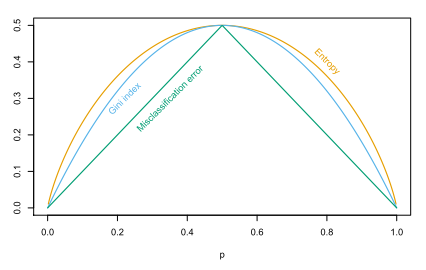
\includegraphics[scale=.5]{ch8_fig1}
\caption{Main reasons regarding why ensemble methods perform better than 
  single models: statistical, computational and representational \citep{Dietterich2000a}.}
\label{fig:8:1}
\end{figure} 
  
  The most typical form of an ensemble is made by combining $T$ different base classifiers.
  Each  base classifier $M(\mathcal{S}_j)$ is trained by applying algorithm $M$ to a random subset 
  $\mathcal{S}_j$ of the training set $\mathcal{S}$.  %  $\mathcal{S_j} = RI(\mathcal{S})$
  For simplicity we define $M_j \equiv  M(\mathcal{S}_j)$ for $j=1,\dots,T$, and 
  $\mathcal{M}=\{M_j\}_{j=1}^{T}$ a set of base classifiers.
  Then, these models are combined using majority voting to create the ensemble $H$ as follows
  \begin{align}\label{eqn:majority-vote}
    f_{mv}(\mathcal{S},\mathcal{M}) = \argmax_{c \in \{0,1\}} \sum_{j=1}^T 
    \mathbf{1}_c(M_j(\mathcal{S})).
  \end{align}

  \newpage
  \begin{remark}{Theoretical performance of an ensemble}
%   Moreover, i
  If we assume that each one of the $T$ base classifiers have a probability $\rho$ of 
  being correct, the probability of an ensemble making the correct decision, denoted by $P_c$,
  can be calculated using the binomial \mbox{distribution \citep{Hansen1990}}
  \begin{equation}\label{eq:prob}
    P_c = \sum_{j>T/2}^{T} {{T}\choose{j}} \rho^j(1-\rho)^{T-j}.
  \end{equation}
  Furthermore, as shown in \citep{Lam1997}, if $T\ge3$ then:
  \begin{itemize}
    \item If $\rho>0.5$, then $ \lim_{T \to  \infty} P_c=1 $
    \item If $\rho<0.5$, then $ \lim_{T \to  \infty} P_c=0 $
    \item If $\rho=0.5$, then $P_c=0.5$ for any $T$.
  \end{itemize}
  Leading to the conclusion that $P_c\ge \rho$ if $\rho \ge 0.5$ for any $T$.
  \end{remark}
  
\subsection{Cost-sensitive ensembles}

  In the context of cost-sensitive classification, some authors have proposed methods for using 
  ensemble techniques. In \citep{Masnadi-shirazi2011}, the authors proposed a framework for 
  cost-sensitive boosting that is expected to minimized the losses by using optimal cost-sensitive 
  decision rules. In \citep{Street2008}, a bagging algorithm with adaptive costs was proposed. In 
  his doctoral thesis, Nesbitt \citep{Nesbitt2010}, proposed a method for cost-sensitive 
  tree-stacking. In this method different decision trees are learned, and then combined in a way 
  that a cost function is minimized. Lastly in \citep{Lomax2013}, a survey of application of 
  cost-sensitive learning with decision trees is shown, in particular including other methods that 
  create cost-sensitive ensembles. However, in all the previously presented method, the 
  misclassification costs only dependent on the class, therefore, assuming a constant cost across 
  examples. Given that, these methods are not  well suited for example-dependent cost-sensitive 
  problems. 

      
\section{Ensembles of cost-sensitive decision trees}
\label{sec:8:ecsdt}

In this section we shown our previously proposed framework of ensembles of  example-dependent 
cost-sensitive  decision-trees \citep{CorreaBahnsen2015b}, by training example-dependent 
cost-sensitive decision trees using four different  random inducer methods and then blending them 
using three different combination approaches. Moreover, we propose two new cost-sensitive 
combination approaches, cost-sensitive weighted  voting and cost-sensitive stacking. The latter 
being an extension of our previously proposed cost-sensitive logistic regression 
\citep{CorreaBahnsen2014b}. 

The remainder of the section is organized as follows: First, we introduce the example-dependent 
cost-sensitive decision tree. Then we present the different random inducers and combination 
methods. Finally, we define our proposed algorithms.
  
 
\section{Theoretical analysis of the ECSDT}
\label{sec:8:theoretical}

    
\section{Experiments}
\label{sec:8:experiments}

\section{Overall experiments}
\label{sec:8:experiments_all}